% Capítulo 2
\chapter{Arash}

\abrv[ARASH -- \textit{Anthropomorphic Robot Augmented with Sense of Human}, em livre tradução Robô Antropomórfico Aumentado com Sentido de Ser Humano]{ARASH}(\textit{Anthropomorphic Robot Augmented with Sense of Human}, em português Robô Antropomórfico Aumentado com Sentido de Ser Humano), é um robô de 7,5 Kg e 1 metro de altura. Possuindo 20 graus de liberdade (ou \abrv[DOF -- Do inglês \textit{Degrees Of Freedom}, ou graus de liberdade]{DOF}, do inglês \textit{degrees of freedom}), ele tenta imitar a configuração humana, tanto em suas juntas quanto em suas proporções. Em suas juntas, Arash possui motores MX-28, MX-64 e MX-106 (da Robotis Co), dependendo da carga suportada. Como controlador principal, um computador \textit{mini-box} é utilizado em conjunto com uma placa microcontroladora \textit{OpenCM9.04} que serve de interface entre o controlador principal e os motores \cite{autdp2016}.

\noindent\makebox[\linewidth]{\rule{\paperwidth}{0.4pt}}

\begin{draft}
	A caminhada de robôs com pernas vem sendo desenvolvida desde da década de 70, quando Kato e Vukobratovic praticamente iniciaram este campo de estudo \cite{kajita2008}.
\end{draft}

\begin{draft}
	\todo{Reescrever esta desgraça}
	\todo{Introduzir os conceitos de equilíbrio estático e dinâmico.}No desenvolvimento de qualquer \textit{walking gait}, é necessário a estratégia de equilíbrio entre estática ou dinâmica. Cada estratégia tem suas vantagens e desvantagens. Todavia, o equilíbrio dinâmico vem sendo mais aceito dentre os pesquisadores.
\end{draft}
	
\begin{draft}
	O equilíbrio estático mantém o centro de massa, ou \abrv[CoM -- Centro de massa, do inglês \textit{Center of Mass}]{CoM -- do inglês \textit{Center of Mass} --} sempre sob a superfície de apoio do robô. Uma enorme desvantagem é que as velocidades alcançadas são bem lentas, tendo em vista que o movimento produzido para a caminhada não deve gerar inercia suficiente para deslocar o CoM fora da área esperada. Geralmente observa-se pés maiores em robôs que adotam este tipo de caminhada \cite{miller1994}.
\end{draft}

\begin{draft}	
	Ainda segundo Miller, o equilíbrio dinâmico, considera a dinâmica do movimento da caminhada, as inércias das partes que movem-se. Com isto, ela habilita o CoM movimentar-se para fora do ponto de apoio, mantendo o robô em uma espécie de ``queda controlada''. Assim, ela habilita maiores velocidades de caminhada com maior eficiência.
\end{draft}

\begin{draft}
	Durante qualquer tarefa envolvendo locomoção é necessária uma maneira de controlar o \textit{walking gait} de forma a direcionar o robô ao destino escolhido. Uma das formas utilizadas são movimentos pré-definidos que executam ações específicas. Assim, essas ações são sequenciadas de forma a levar o robô até seu destino. Por exemplo, dar um passo a frente, um passo lateral à esquerda, girar 30\degree à direita. A desvantagem deste método é que cada ação deve ser executada em sequência, o que pode levar a menos agilidade.
\end{draft}

\begin{draft}
	Uma segunda forma de controle é a chamada caminhada omnidirecional que consiste em controlar o robô por velocidades em diferentes eixos. Essas mudanças podem ser realizadas com o robô em movimento, sem a necessidade de encadeamento de ações. Adicionalmente, existe a possibilidade de combinar movimentos em diferentes eixos ao mesmo tempo criando novas possibilidades de locomoção e aumentando a agilidade do robô.
\end{draft}

\noindent\makebox[\linewidth]{\rule{\paperwidth}{0.4pt}}

\subsection{Graus de Liberdade e Atuadores}
\label{subsec:architecture:Atuators}

\todo{Adicionar um parágrafo introdutório.}
PARAGRAFO INTRODUTÓRIO.

Os DOFs são o número de parâmetros de posições independentes que definem a configuração de uma sistema mecânico \cite{craig1989} e tão importante quanto sua configuração é a sua orientação para que os cálculos funcionem como o esperado. A inversão de qualquer orientação entre o modelo matemático e o modelo real causará uma inversão durante a caminhada, causando reações inesperadas e possíveis danos aos motores.

\begin{figure}[htb]
	\centering
	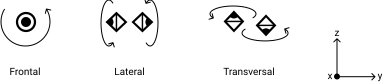
\includegraphics[scale=1]{imagens/svg/actuators-orientation}
	\caption{Orientação dos movimentos dos atuadores}
	\label{fig:ActuatorsOrientation}
\end{figure}

A figura~\ref{fig:ActuatorsOrientation} exibe as possíveis orientações dos atuadores que são referenciadas ao longo do trabalho como frontal, lateral e transversal.

Atuadores com orientação frontal -- ou simplesmente, atuadores frontais -- propiciam rotação orientada pelo eixo $X$, que está aponta para o leitor (para fora do papel). Esse tipo de rotação também é referida como \textit{roll}.

Atuadores laterais apontam para direita ou esquerda. Eles apresentam rotação com base no eixo $Y$ (plano $XZ$), também conhecida como rotação \textit{pitch}. Analogamente, atuadores transversais apontam para cima ou baixo, com base no eixo $Z$ (plano $XY$), com movimento de rotação conhecido como \textit{yaw}.

Na figura~\ref{fig:architecture:arash:actuators_orientations}, observa-se o esquema de orientação dos atuadores aplicada no diagrama das juntas de Arash. Ainda na mesma figura, os ``triângulos pretos preenchidos'' representam apenas o fim de uma cadeia de atuadores. Assim, estes símbolos representam as mãos, que não possuem atuadores, e a ponta da cabeça, onde encontra-se a câmera. 

\begin{figure}[htb]
	\centering
	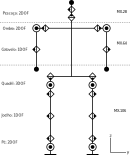
\includegraphics[scale=1]{imagens/svg/arash-schematics}
	\caption{Diagrama de orientação dos atuadores de Arash}
	\label{fig:architecture:arash:actuators_orientations}
\end{figure}

Em Arash, todos os atuadores utilizados são produzidos pela Robotics.Co. Porém, devido a variação de carga nas diversas juntas, foram utilizados diferentes modelos da série MX. Esta decisão de projeto diminui bastante o custo final do robô.

No pescoço, onde a carga é bem leve, ``MX-28'' são suficientes. Dois atuadores, um na posição transversal (o atuador mais baixo) que fornece o movimento panorâmico a cabeça e outro na posição horizontal, fornecendo o movimento de inclinação vertical da cabeça.

Nos braços, que podem sofrer uma carga maior, atuadores ``MX-64'' são utilizados. Isso é importante já que existem modalidades de competições, como o levantamento de peso, que testam a capacidade do carregamento de cargas.

Para as pernas, foram utilizados atuadores ``MX-106'' que são mais poderosos que os anteriores. Entretanto, na fase de projeto, simulações mostraram que durante o movimento de levantar-se do chão (em caso da recuperação de uma possível queda), o torque nas juntas do joelho era levado ao máximo suportado pelo ``MX-106'', podendo assim levar este motor à falha. Desta forma, 2 atuadores sincronizados passaram a formar esta junta, afim de compartilhar a carga sofrida entre dois motores. Esta junta dupla não oferece nenhum impacto na implementação, já que os motores da série ``MX-106'' oferecem a capacidade de serem ligados e sincronizados via \textit{hardware}. Assim, a nível de software controla-se apenas 1 único atuador. Desta forma, apesar das 20 DOF, Arash possui 22 motores.